\section{Analysis}



	\subsection{Quiz Scores}
		There are 4 games with quizzes, each with 20 responses each, 80 responses total. I graded each pre- and post-quiz, and ended up with the percent change for each response. After averaging these changes, I found that, after playing an educational game for a short period of time, the average player's score went up by 3\%.

		For the number of responses I've received, this is not a statistically signficant number. I could allocate more surveys, get hundreds or thousands more responses in order to try to make it significant, but my efforts are better spent trying to make a more accurate survey.

		\subsubsection{Statistical Significance using t-distributions}

			\begin{figure}[h] 
				\centering 
				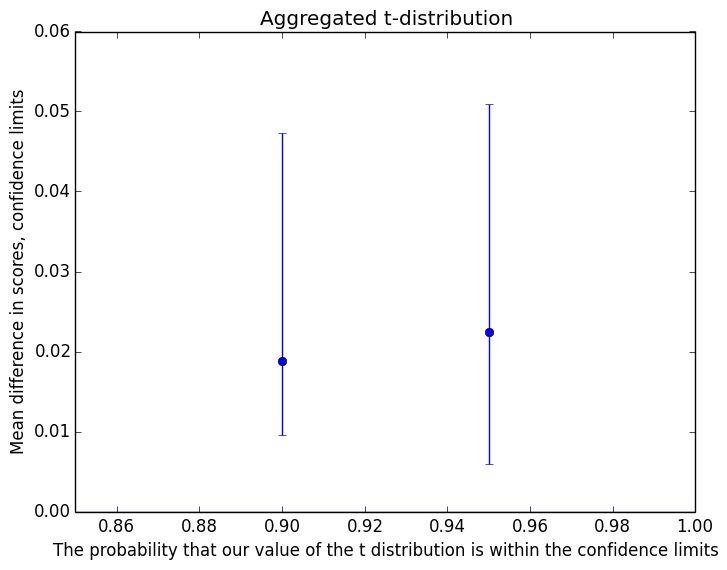
\includegraphics[width=\textwidth]{aggregated_tdist.png} 
				\caption{Aggregated tdist}
			\end{figure}
			\begin{figure}[h] 
				\centering 
				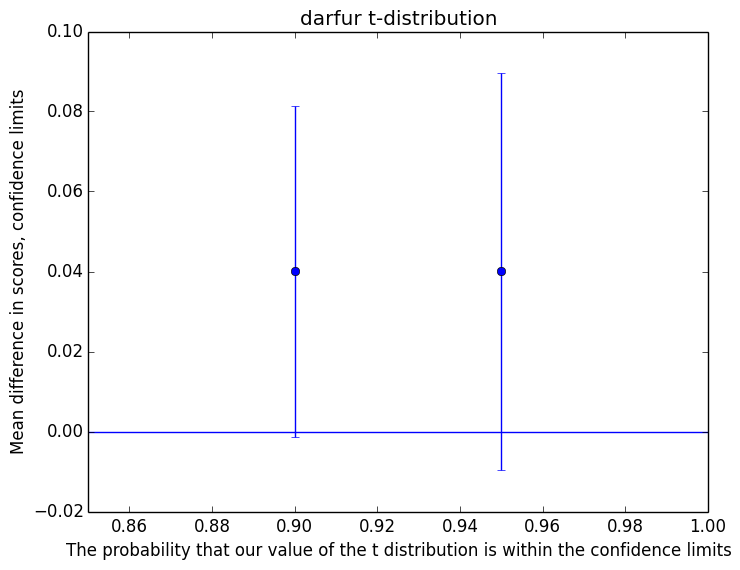
\includegraphics[width=\textwidth]{darfur_tdist.png} 
				\caption{Darfur tdist}
			\end{figure}
			\begin{figure}[h] 
				\centering 
				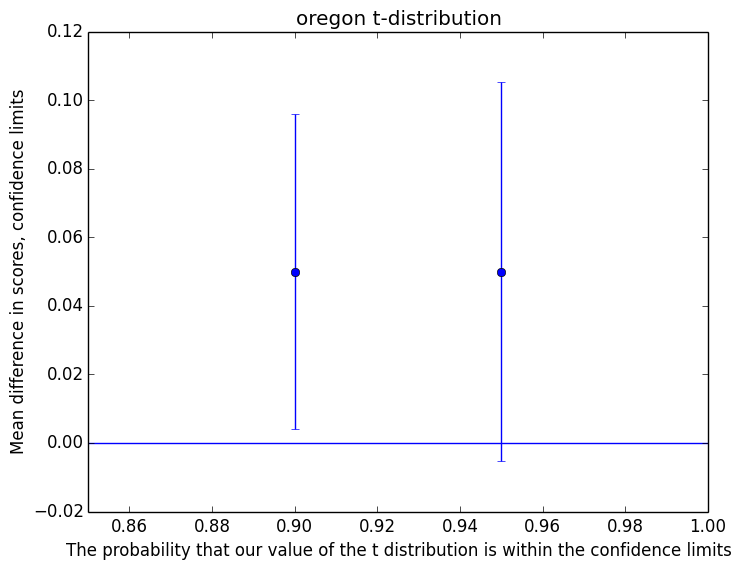
\includegraphics[width=\textwidth]{oregon_tdist.png} 
				\caption{Oregon tdist}
			\end{figure}
			\begin{figure}[h] 
				\centering 
				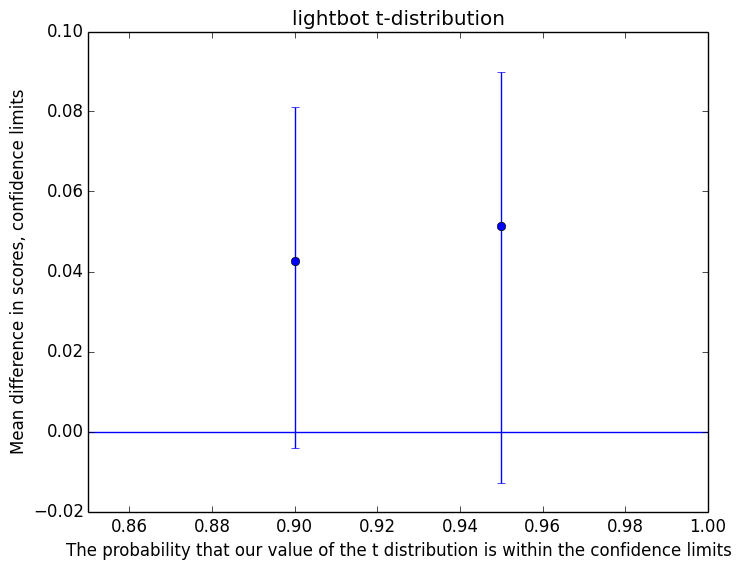
\includegraphics[width=\textwidth]{lightbot_tdist.png} 
				\caption{Lightbot tdist}
			\end{figure}
			\begin{figure}[h] 
				\centering 
				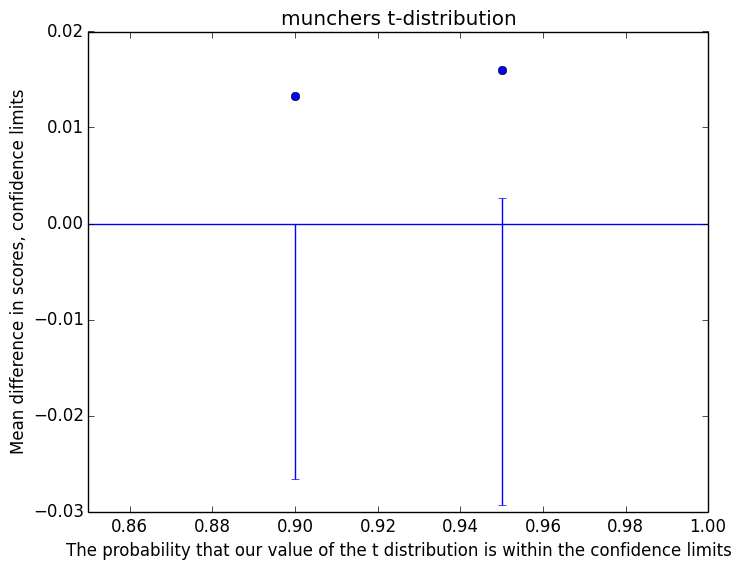
\includegraphics[width=\textwidth]{munchers_tdist.png} 
				\caption{Munchers tdist}
			\end{figure}

		\subsubsection{Rubric Inter-rater Reliability}
			\begin{figure}[h] 
				\centering 
				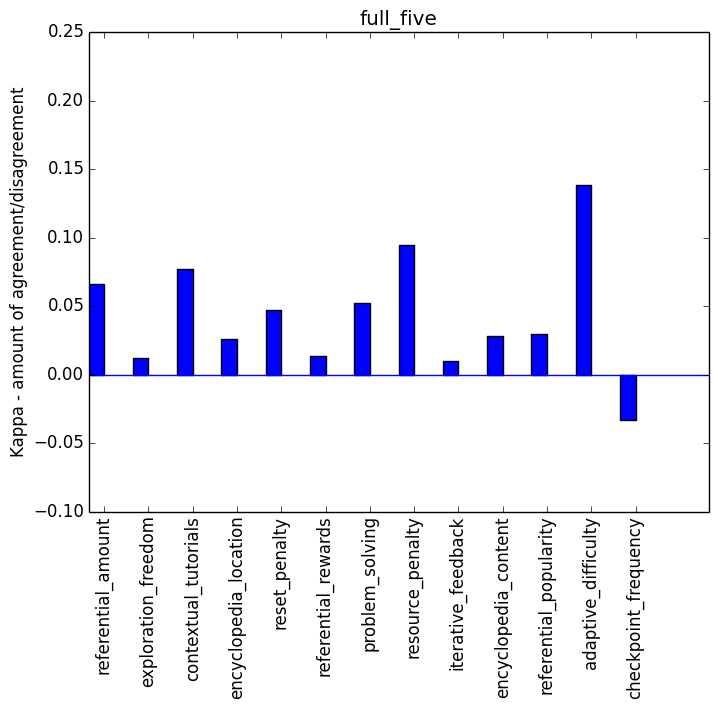
\includegraphics[width=\textwidth]{full_five_stats.png} 
				\caption{Inter-rater reliability}
			\end{figure}
			\begin{figure}[h] 
				\centering 
				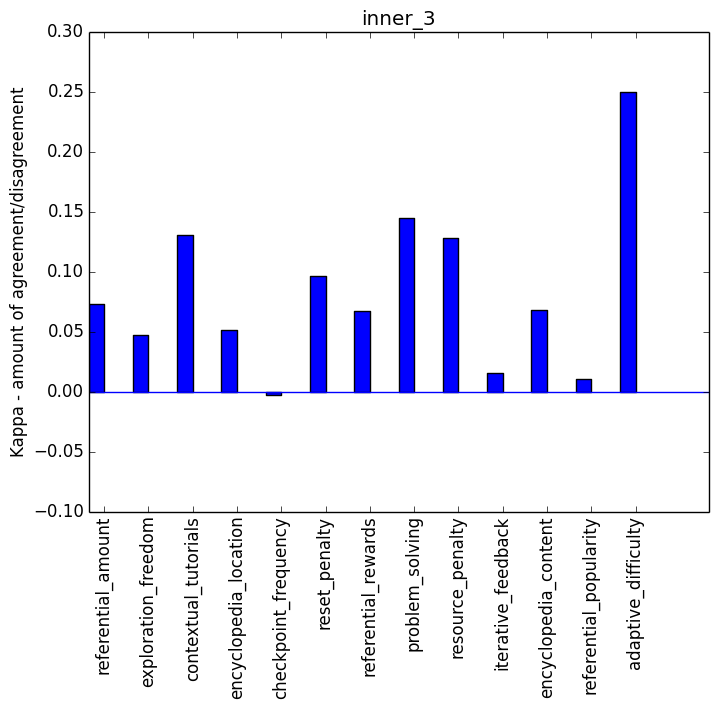
\includegraphics[width=\textwidth]{inner_3_stats.png} 
				\caption{Inter-rater reliability with middle 3 options combined}
			\end{figure}
			\begin{figure}[h] 
				\centering 
				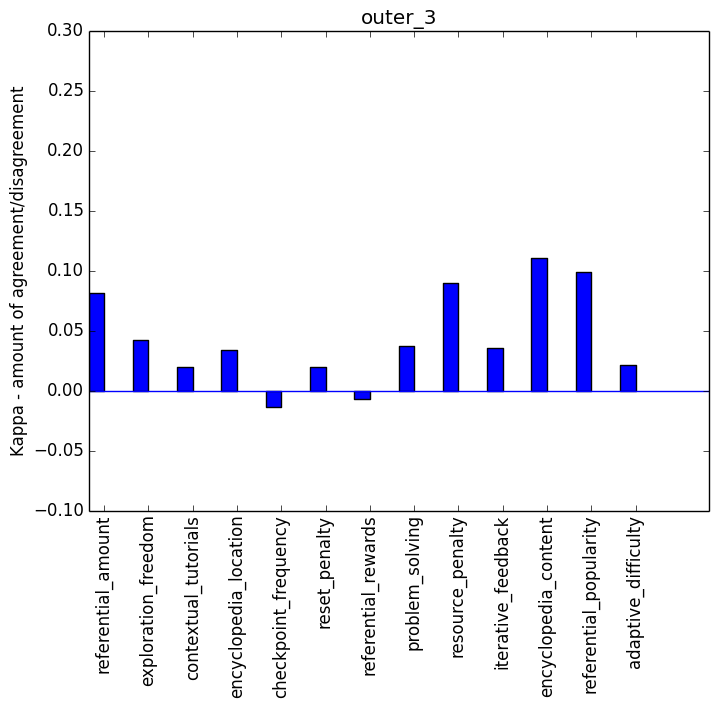
\includegraphics[width=\textwidth]{outer_3_stats.png} 
				\caption{Inter-rater reliability with outer pairs combined}
			\end{figure}

		\subsubsection{Quiz Postmortem}
			There are a number of reasons why the results may have fallen so flat.

			The quiz itself may have been faulty; perhaps the questions were too hard, too easy, or covered content that was not taught as part of the game. To combat this, the quizzes were designed to cover material that players were supposed to learn in the game, but it's possible that the multiple-choice format wasn't the best way to do that.

			It's also possible that the games weren't actually effective in teaching the players anything at all. Because of how the games were designed, players didn't retain any relevant information about what the game was trying to educate them on.

			Another option is that the platform on which the surveys were administered has faults. There are spammers on Mechanical Turk, and while it is possible to review and reject responses deemed unusable, it's impractical to filter out every single one. However, if a spammer is selecting random responses, it's highly unlikely that they'll end up with a higher or lower score than when they started. 

			It's also possible to filter out poorly rated workers with an ``acceptance rate" criteria, where Workers that accept the task are required to have at least a 90\% acceptance rate across all of their HITs, but that increases response times and payout amounts.

			Finally, it's possible that some workers lost interest in the HIT once they had finished the first sections, resulting in shoddy work on the second. This would mean that some workers would guess at the questions in the post-quiz, resulting in worse performance across the board.

			For a future quiz/survey on the Mechanical Turk platform, I'd recommend both an ``acceptance rate" criteria, as well as some form of automated validation that the worker is actually completing the survey. This may include a ``dummy question," where the reviewer only has to click the right button, or some other kind of verification where they submit a screenshot of their highest score within the game. This will increase response times and require higher payout amounts, but if it's focused only on one game it won't be much.

			Another route worth exploring is paying out ``bonuses" to workers who show exemplary work in the quiz and survey. However, you'd have to make sure to incentivize honesty and not greed; my hunch is that asking workers to not use the internet to find solutions may not work when there's extra payouts involved.











